\documentclass[12pt]{article}
\usepackage[utf8]{inputenc}
\usepackage{graphicx}
\usepackage{amsmath}
\usepackage{amsfonts}

\title{DD Lab 2 Assignment}
\author{Sai Kartik \\2020A3PS0435P}

\begin{document}
\maketitle
\section{Realisation with multi-input NAND gates}
\begin{center}
    \begin{figure}[ht]
        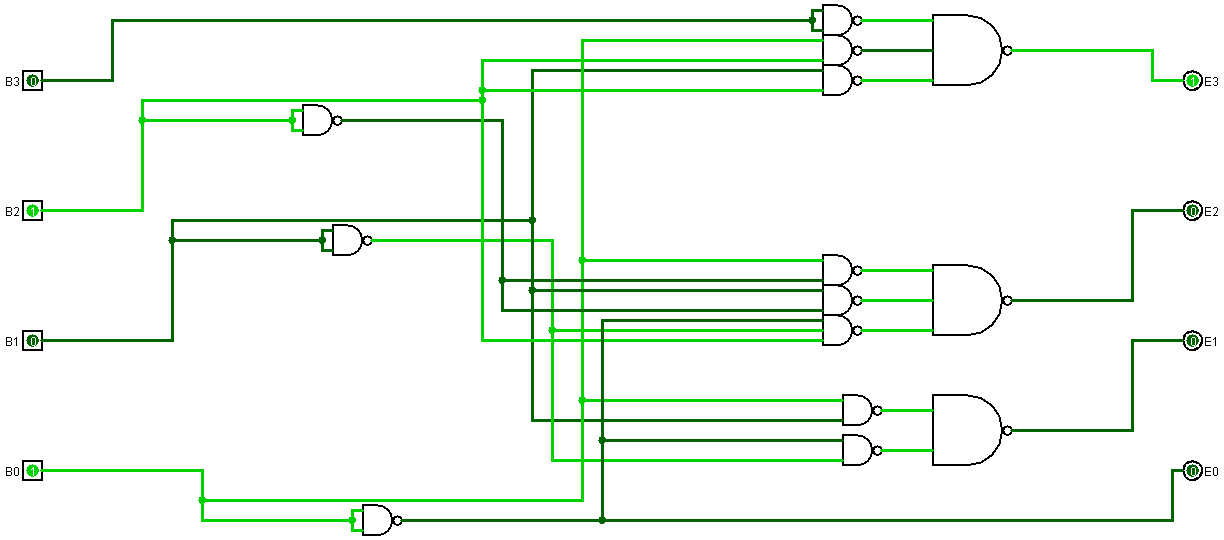
\includegraphics[scale=0.30]{onlynands.png}
        \caption{BCD to Excess 3 converter realised with only NAND gates (multiple-input gates)}
    \end{figure}
\end{center}
\newpage
\subsection{Truth Table generated}
\begin{center}
    \begin{figure}[ht]
        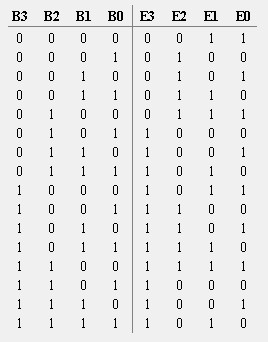
\includegraphics{ttonlynands.jpg}
        \caption{Truth table for the above realisation}
    \end{figure}
\end{center}
\subsection{Simplified expressions for this realisation}
$$E_0=\bar{B}_0$$
$$E_1=B_0B_1+\bar{B}_0\bar{B}_1 $$
$$E_2=B_0\bar{B}_2+B_1\bar{B}_2+\bar{B}_0\bar{B}_1B_2$$
$$E_3=B_3+B_0B_2+B_1B_2$$
\newpage
\section{Realisation with only 2-input NAND gates}
\begin{center}
    \begin{figure}[ht]
        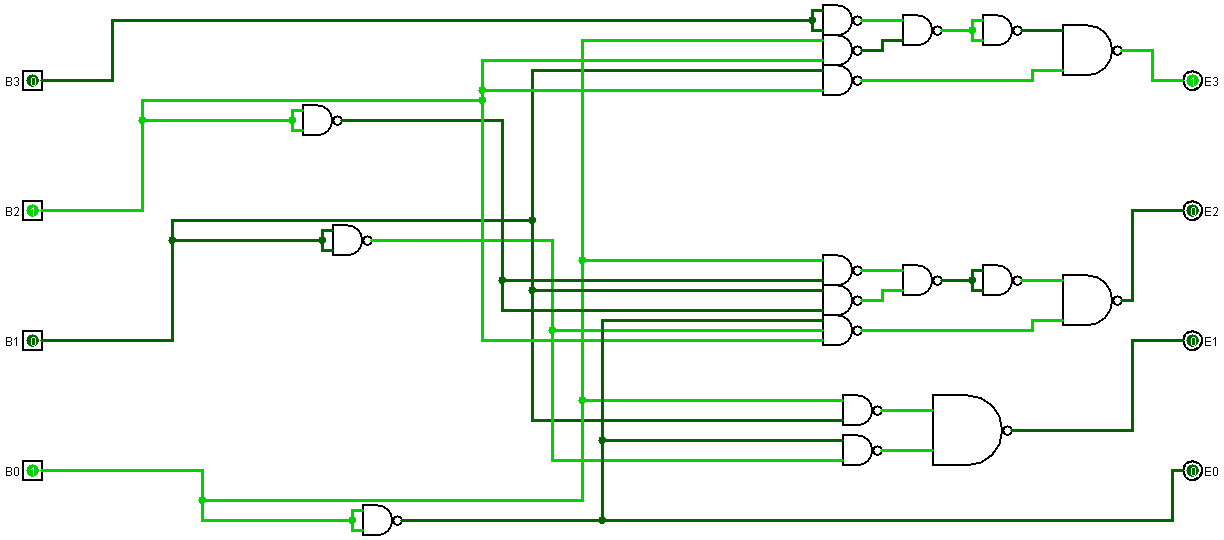
\includegraphics[scale=0.30]{only2nands.png}
        \caption{BCD to Excess 3 converter realised with only NAND gates (only 2-input gates)}
    \end{figure}
\end{center}
\newpage
\subsection{Truth Table generated}
\begin{center}
    \begin{figure}[ht]
        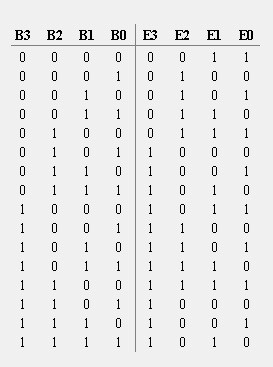
\includegraphics{ttonly2nands.jpg}
        \caption{Truth table for the above realisation}
    \end{figure}
\end{center}
\newpage
\section{Realisation with multi-input NOR gates}
\begin{center}
    \begin{figure}[ht]
        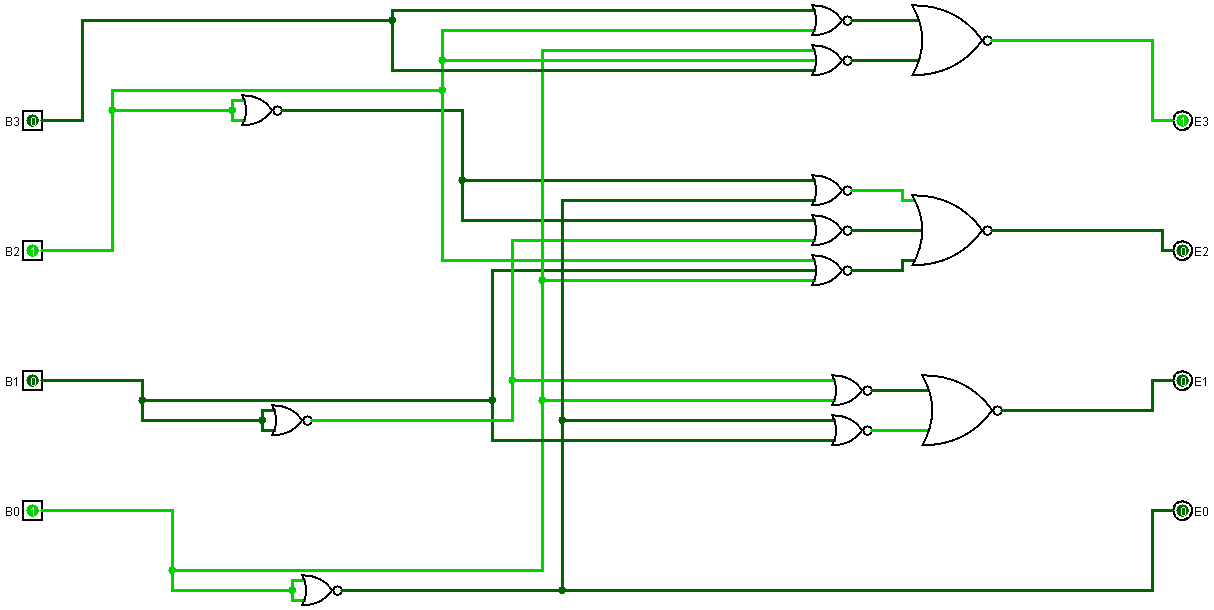
\includegraphics[scale=0.30]{onlynors.png}
        \caption{BCD to Excess 3 converter realised with only NOR gates (multiple-input gates)}
    \end{figure}
\end{center}
\newpage
\subsection{Truth Table generated}
\begin{center}
    \begin{figure}[ht]
        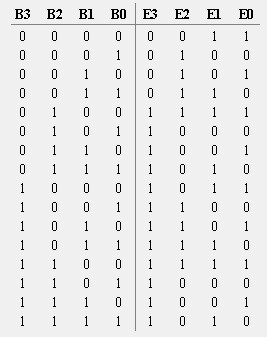
\includegraphics{ttonlynors.jpg}
        \caption{Truth table for the above realisation}
    \end{figure}
\end{center}
\subsection{Simplified expressions for this realisation}
$$E_0=\bar{B}_0$$
$$E_1=(\bar{B}_0+B_1)(B_0+\bar{B}_1)$$
$$E_2=(\bar{B}_0+\bar{B}_2)(\bar{B}_1+\bar{B}_2)(B_0+B_1+B_2)$$
$$E_3=(B_0+B_1+B_3)(B_2+B_3)$$
\newpage
\section{Realisation with only 2-input NOR gates}
\begin{center}
    \begin{figure}[ht]
        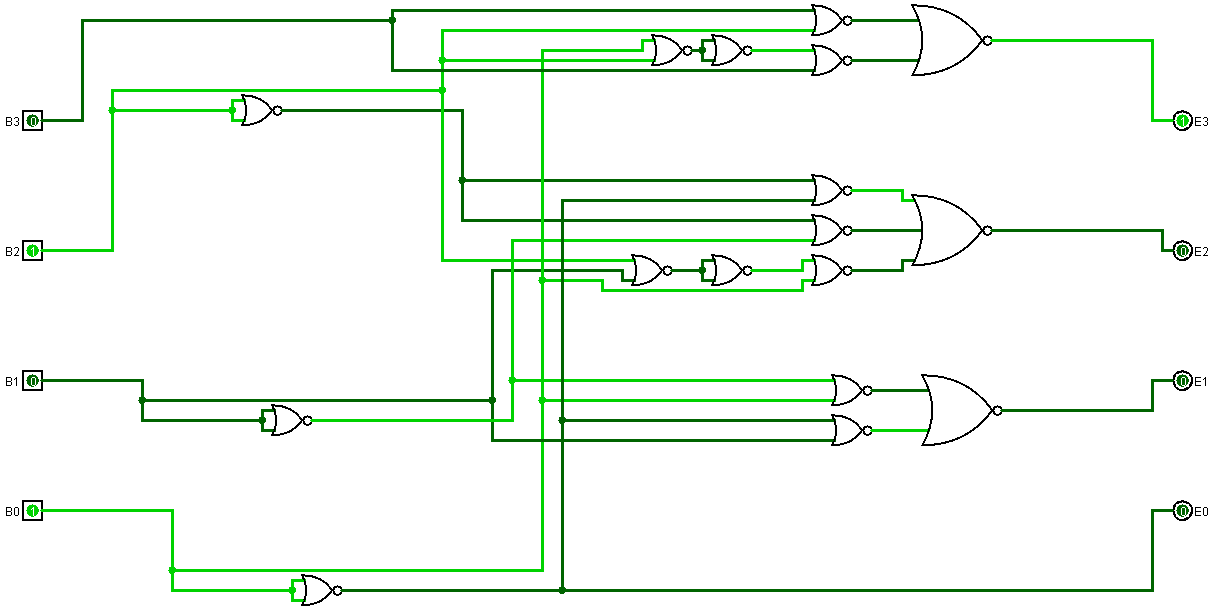
\includegraphics[scale=0.30]{only2nors.png}
        \caption{BCD to Excess 3 converter realised with only NOR gates (only 2-input gates)}
    \end{figure}
\end{center}
\newpage
\subsection{Truth Table generated}
\begin{center}
    \begin{figure}[ht]
        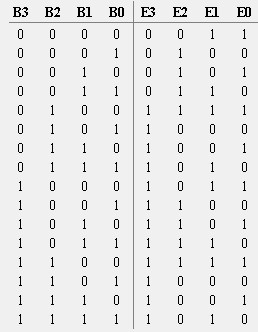
\includegraphics{ttonly2nors.jpg}
        \caption{Truth table for the above realisation}
    \end{figure}
\end{center}
\end{document}